\vskip3mm
   {\bf Partie A} \par \smallskip
   Dans une école, un jardin pédagogique est constitué d’un terrain rectangulaire $ABEC$ dont l’aire est égale à \Aire[m]{100}. \par \smallskip
   Des enseignants de l’école décident de planter avec les élèves différentes cultures sur ce terrain : des fraisiers, des pieds de tomates et des radis. \par
   La répartition dans le terrain est la suivante :
   \begin{center}
      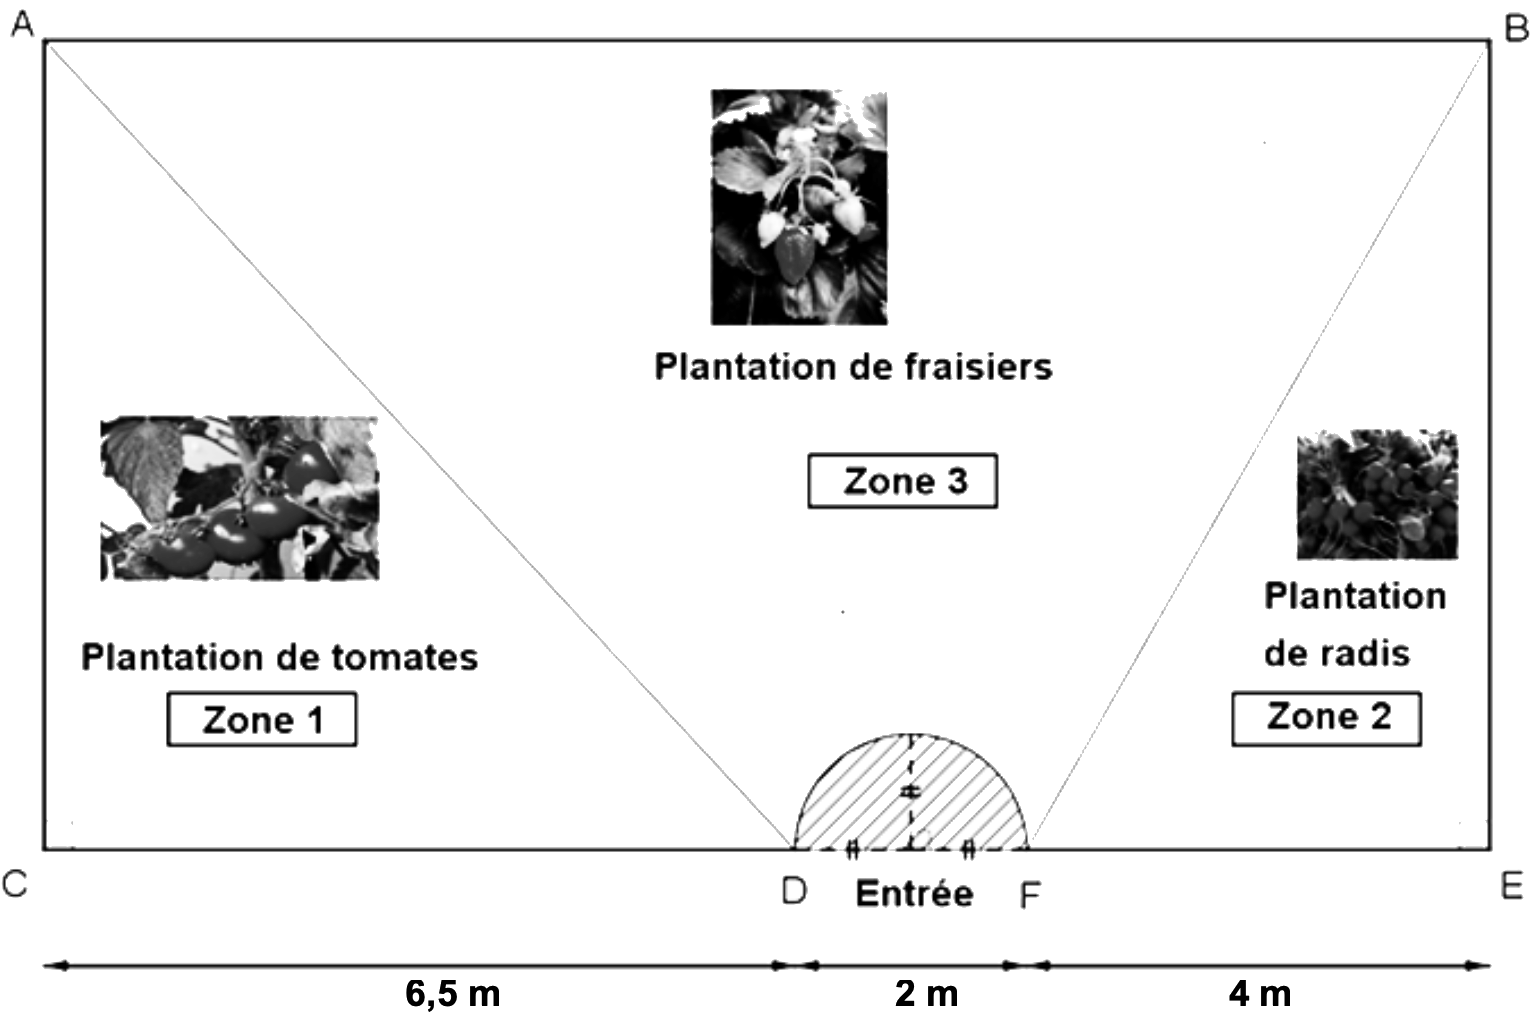
\includegraphics[width=15cm]{Images/Plantations}
   \end{center}
   L’entrée est un demi-disque délimité par le demi-cercle de diamètre $[DF]$ (zone hachurée sur la figure ci-dessus). Elle doit rester libre de toute plantation.
   \begin{enumerate}
      \setlength{\itemsep}{-1mm}
      \item Justifier que la largeur du terrain correspondant au segment $[CA]$ est égale à \Lg[m]{8}.
      \item Tracer un plan du terrain avec les différentes zones à l’échelle 1 : 80.
      \item Le directeur de l’école veut installer une bordure sur les trois côtés autour de la zone 1 où on plante des tomates.
         \begin{enumerate}
            \setlength{\itemsep}{-1mm}
            \item Montrer que $AD =\sqrt{106,25}$ m.
            \item Déterminer la longueur de la bordure qu’il doit acheter. On donnera le résultat en mètre, arrondi à l’unité.
            \item Les bordures sont vendues par rouleaux de 4 mètres. Déterminer le nombre de rouleaux nécessaire pour entourer la zone 1.
         \end{enumerate}
      \item On veut déterminer l’aire de chacune des zones.
         \begin{enumerate}
            \setlength{\itemsep}{-1mm}
            \item Calculer l’aire de la zone 1, en mètre carré.
            \item Calculer l’aire de la zone 2, où on plante des radis, en mètre carré.
            \item En déduire l’aire de la zone 3, où on plante des fraisiers (sans la zone << Entrée >> hachurée sur la figure), en mètre carré. Donner la valeur exacte puis la valeur arrondie au dixième.
         \end{enumerate}
      \item On s’intéresse à la culture des fraisiers. Sachant qu’on peut planter 6 pieds de fraisiers par m2 et qu’un pied de fraisier produit en moyenne 650 grammes de fraises par année, quelle masse de fraises les élèves peuvent- ils espérer récolter ? On donnera le résultat en kilogramme, arrondi à l’unité.
   \end{enumerate}

   \vskip2mm
   {\bf Partie B} \par \smallskip
   Fin juin, l’école décide de récolter des fraises pour faire de la confiture. Les élèves récoltent ainsi \Masse[kg]{25} de fraises.
   \begin{enumerate}
      \setlength{\itemsep}{-1mm}
      \item La recette de confiture de fraise dit que la quantité de sucre nécessaire doit correspondre à 55\,\% de la masse totale avant cuisson. Quelle masse de sucre, arrondi au kilogramme, le directeur doit-il acheter pour respecter cette recette ?
      \item Sachant que \Masse[kg]{3} de fraises permettent de réaliser \Capa{4,8} de confiture, combien de litres de confiture peut-on réaliser ?
      \item Il décide de conditionner cette confiture dans des pots cylindriques dont la base est un disque de diamètre \Lg{8,4} et dont la hauteur mesure \Lg{11}. Sachant que les pots ne peuvent être remplis qu’au 8/9 de leur capacité maximale, déterminer le nombre de pots de confiture qu’il devrait réaliser. \par
        {\it On rappelle la formule suivante : Volume d'un prisme ou d'un cylindre : $V=B\times h$, \newline
        où $B$ désigne l’aire de la base du prisme ou du cylindre et $h$ sa hauteur.}
   \end{enumerate}